\fancyfoot[C]{G�rel}
\subsubsection{Versionsverwaltung}
Versionsverwaltungssysteme erm�glichen Entwicklern, den Verlauf ihres Codes zu verfolgen, �nderungen zu verwalten und problemlos zusammenzuarbeiten. Unter den verschiedenen Optionen f�r Versionsverwaltung ist GitHub eine der am weitesten verbreiteten Plattformen, die von Millionen von Entwicklern weltweit genutzt wird.

\paragraph{Historie und R�ckverfolgbarkeit: }
Ein zentrales Merkmal von Versionsverwaltungssystemen ist die F�higkeit, den Verlauf aller �nderungen am Code zu verfolgen. Entwickler k�nnen durch die gesamte Historie des Projekts navigieren, um zu sehen, wer welche �nderungen vorgenommen hat und wann diese durchgef�hrt wurden. Dies erm�glicht eine detaillierte R�ckverfolgbarkeit und erleichtert das Debugging und die Fehlerbehebung. Da nur die Ver�nderung am Code gespeichert wird, ist diese Art der Versionsverwaltung besonders effizient, da nicht f�r jede Version die komplette Datei neu gespeichert werden muss.

\paragraph{Zusammenarbeit und Teamarbeit: }
Versionsverwaltungssysteme erm�glichen eine effiziente Zusammenarbeit zwischen Entwicklern, auch wenn sie an verschiedenen Standorten arbeiten. Mehrere Entwickler k�nnen gleichzeitig am gleichen Projekt oder Code arbeiten, ohne sich gegenseitig zu st�ren. Durch die M�glichkeit, Branches zu erstellen und Merge-Anfragen zu stellen, k�nnen Entwickler ihre Arbeit isoliert voneinander durchf�hren und dann problemlos in den Hauptcode integrieren.

\paragraph{Branches und Forks: }
\textbf{Branches} sind Kopien des Codes, die unabh�ngig voneinander entwickelt werden k�nnen. Benutzer k�nnen Branches erstellen, um neue Funktionen zu implementieren oder Fehler zu beheben, ohne den Hauptcode zu modifizieren. Der Hauptcode wird in einem sogenannten "Master" -Branch verwaltet, w�hrend Entwickler f�r jede neue Funktion oder �nderung einen eigenen Branch erstellen k�nnen. Dies erm�glicht es, dass mehrere Entwickler gleichzeitig an verschiedenen Funktionen arbeiten k�nnen, ohne sich gegenseitig zu st�ren. Nachdem die Arbeit an einem Branch abgeschlossen ist und alle Tests erfolgreich durchgef�hrt wurden, kann der Branch mit dem Hauptcode (Master-Branch) fusioniert werden, um die �nderungen zu integrieren. Dieser Prozess wird als "Merge" bezeichnet und erm�glicht eine geordnete und effiziente Entwicklung von Softwareprojekten.
\begin{figure}[H]
    \centering
    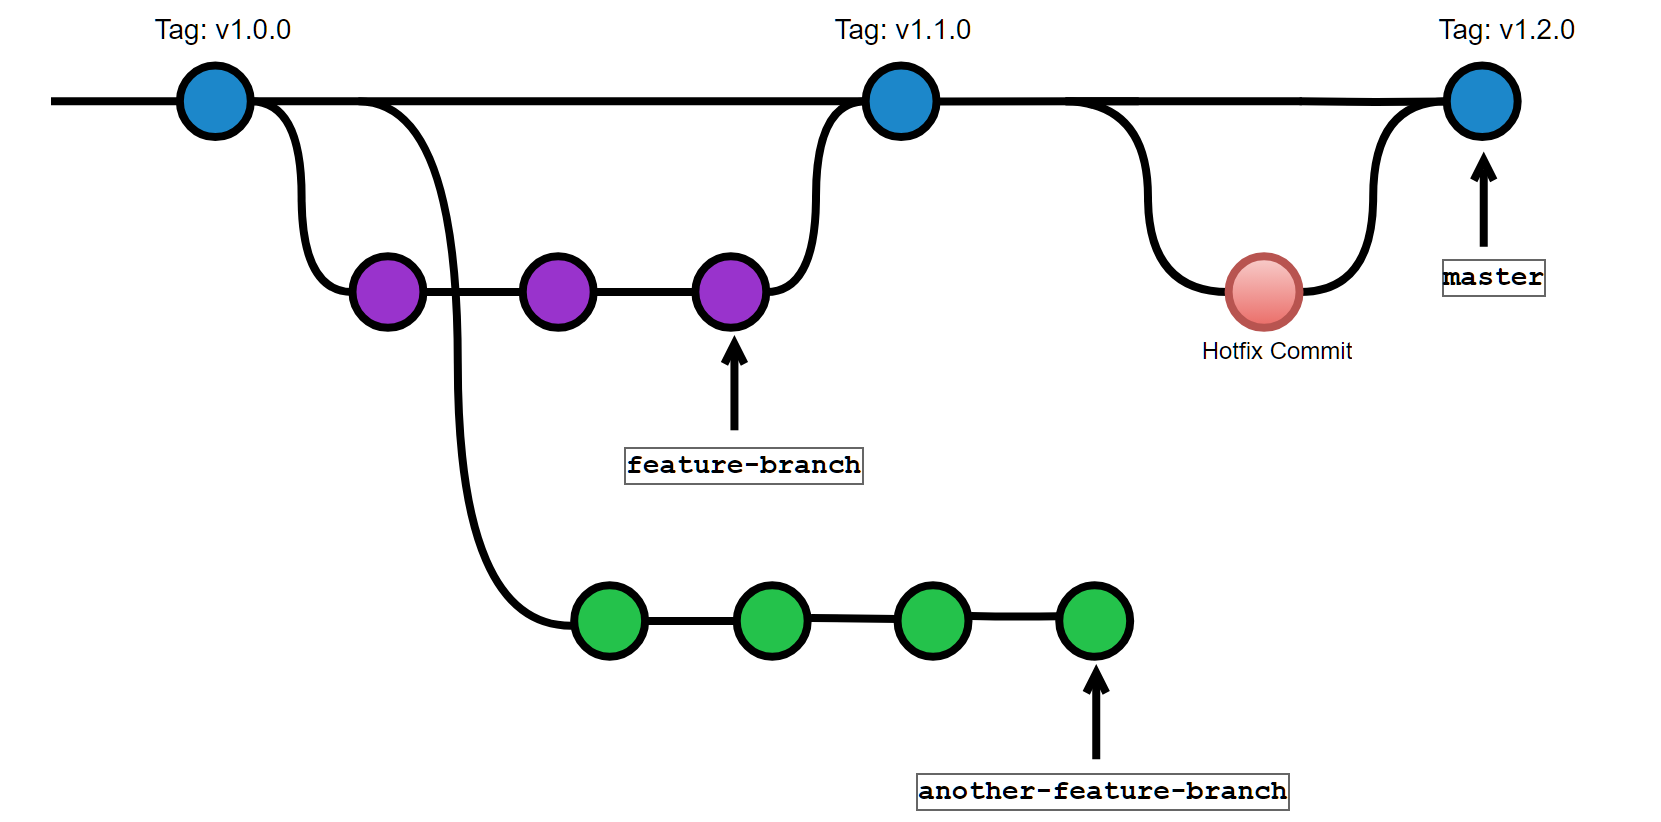
\includegraphics[scale=0.2]{./3_Stand_der_Technik/Abbildungen/git_branch.png}
    \caption{Illustration vom aufbau einer Branch \cite{Capes2018}}
\end{figure}
\textbf{Forks} sind Kopien des gesamten Repositorys, die von einem anderen Entwickler erstellt werden. Sie erm�glichen es Entwicklern, �nderungen vorzunehmen und dann eine Merge-Anfrage zu stellen, um ihre �nderungen in das urspr�ngliche Repository einzubringen. Oft werden Forks auch daf�r genutzt um ein neues Projekt basierend auf dem Basisprojekt zu erstellen. Hierbei muss wieder die Lizenz beachtet werden.
